\section{Toepassing}

\textit{In dit hoofdstuk wordt de vraag ``Waarvoor wordt Blockchain technologie gebruikt?'' beantwoord. Deze vraag is opgesteld omdat er geen toepassing bekend is voor de te realiseren Blockchain onderdelen, zoals aangegeven in de beschrijving van de aanpak. Het antwoord op deze vraag dient om de opdrachtgever te informeren in wat er mogelijk is met Blockchain technologie om zo een toepassing te kiezen voor het te ontwikkelen Proof of Concept. \\ \\ Er is in het bijzonder aandacht geschonken aan Blockchain als development platform aangezien de opdrachtomschrijving, bijlage \ref{appendix:opdrachtformulering}, spreekt over de realisatie van het onderdeel Smart Contract. Uitleg over het onderdeel \glspl{smart_contract} is beperkt gebleven aangezien het buiten de scope van de opdracht valt.
}

Blockchain technologie wordt steeds vaker toegepast voor het opzetten van een gedecentraliseerd systeem. Aangezien de bekendste toepassing van blockchain technologie een financieel systeem is wordt het vaak gezien als technologie die specifiek bedoeld is om financiële diensten te ondersteunen. In de literatuur wordt er echter veel geëxperimenteerd en gespeculeerd over andere mogelijke toepassingen van blockchain technologie.

\begin{wrapfigure}{r}{0.5\textwidth}
  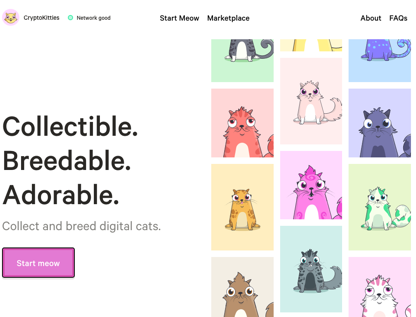
\includegraphics{figures/cryptokitties}
  \caption{CryptoKitties, een spel dat gebruik maakt van Blockchain technologie.}
  \label{cryptokitties}
\end{wrapfigure}

Zo stelt \citeauthor{atzori2015blockchain}, (\citeyear{atzori2015blockchain}) bijvoorbeeld dat blockchain technologie ingezet kan worden om de politiek en de maatschappij te veranderen. In een andere studie gedaan door \citeauthor{crosby2016blockchain}, (\citeyear{crosby2016blockchain}) wordt er onderscheid gemaakt tussen financiële en niet-financiële toepassingen die mogelijk veranderd kunnen worden door blockchain technologie. Een aantal voorbeelden die gegeven worden zijn de toepassingen bij verzekeringen, gedecentraliseerde opslag en domeinregistratie. In fig. \ref{cryptokitties} is een afbeelding te zien van de website van CryptoKitties, een van de eerste spellen die gebruik maakt van blockchain technologie, namelijk het Ethereum netwerk.

\clearpage
\subsection{Ontwikkelplatform}
Blockchains als Ethereum, EOS en HyperLedger bieden hun functionaliteit aan als development platform. Het stelt ontwikkelaars in staat om hun eigen toepassingen te realiseren, zogenaamde \gls{dapps}.

\begin{lstlisting}[
  linewidth=\textwidth, breaklines=true, 
  basicstyle=\small, label={smart_contract},
  caption={Smart contract voor ``The Greeter'' geschreven in Solidity, zoals gepresenteerd in een tutorial voor Smart Contracts op het Ethereum netwerk \citep{ethereum_smart_contract}.}]
  contract Mortal {
    /* Define variable owner of the type address */
    address owner;

    /* This function is executed at initialization and sets the owner of the contract */
    function Mortal() { owner = msg.sender; }

    /* Function to recover the funds on the contract */
    function kill() { if (msg.sender == owner) selfdestruct(owner); }
  }

  contract Greeter is Mortal {
    /* Define variable greeting of the type string */
    string greeting;

    /* This runs when the contract is executed */
    function Greeter(string _greeting) public {
        greeting = _greeting;
    }

    /* Main function */
    function greet() constant returns (string) {
        return greeting;
    }
  }
\end{lstlisting}

Door het gebruik van \glspl{smart_contract}, te zien in fig. \ref{smart_contract}, is het mogelijk om functionaliteit bij transacties te voegen om extra handelingen, die niet gerelateerd zijn tot de kern van een Blockchain implementatie, uit te voeren. Hieronder is een voorbeeld gegeven wat er mogelijk is met betrekking tot \gls{dapps}.

\paragraph{CryptoKitties} is een spel dat gebruikt maakt van het Ethereum platform, bestaand uit verzamelbare en fokbare digitale katten. De uitwisseling en het fokken van CryptoKitties wordt vastgelegd in het Ethereum netwerk door middel van \glspl{smart_contract}. Wanneer twee CryptoKitties gefokt worden, wordt het uiterlijk en de eigenschappen van hun nageslacht bepaald door het 256-bits genoom van elke ouder en een toeval element, wat leidt tot 4 miljard mogelijke genetische variaties \citep{cryptokitties}.
